\documentclass[11pt]{beamer}
\usepackage{listings} % Include the listings-package
\usepackage[T1]{fontenc}
\usepackage[utf8]{inputenc}
\usepackage[english]{babel}
\usepackage{amsmath}
\usepackage{amssymb, amsfonts, latexsym, cancel}
\usepackage{float}
\usepackage{graphicx}
\usepackage{epstopdf}
\usepackage{subfigure}
\usepackage{hyperref}
%\usepackage{authblk}
\usepackage{blindtext}
\usepackage{booktabs} % Allows the use of \toprule, 
\usepackage{filecontents}
\usepackage{courier} %% Sets font for listing as Courier.
\usepackage{listings}
\usepackage{multicol}



%\usepackage{listings, xcolor}
\lstset{
tabsize = 2, %% set tab space width
showstringspaces = false, %% prevent space marking in strings, string is defined as the text that is generally printed directly to the console
numbers = left, %% display line numbers on the left
commentstyle = \color{green}, %% set comment color
keywordstyle = \color{blue}, %% set keyword color
stringstyle = \color{red}, %% set string color
rulecolor = \color{black}, %% set frame color to avoid being affected by text color
basicstyle = \small \ttfamily , %% set listing font and size
breaklines = true, %% enable line breaking
numberstyle = \tiny,
}
\usepackage{caption}
\DeclareCaptionFont{white}{\color{white}}
\DeclareCaptionFormat{listing}{\colorbox{gray}{\parbox{\textwidth}{#1#2#3}}}
\captionsetup[lstlisting]{format=listing,labelfont=white,textfont=white}
\definecolor{urlColor}{rgb}{0.06, 0.3, 0.57}
\definecolor{linkColor}{rgb}{0.57, 0.0, 0.04}
\definecolor{fileColor}{rgb}{0.0, 0.26, 0.26}
\hypersetup{
    colorlinks=true,
    linkcolor=linkColor,
    filecolor=fileColor,      
    urlcolor=urlColor,
}
\urlstyle{same}
\setbeamercovered{transparent}
%\usetheme{Boadilla}
\usetheme{CambridgeUS}
%\usetheme{Berkeley}
%\usetheme{Warsaw}
%\usetheme{Madrid}

\title[Experiencia de Usuario]{\bf\Huge Experiencia de usuario en portales web}

\author[Grupo 09]
{
	César Paul Vasquez Alvarez \\
	Christian Gonzalo Layme Fernandez \\
	Emerson Danny  Mendoza Hilasaca \\
	Edith Maricarmen Coaquira Cuevas  
}
\institute[UNSA]
{
System Engineering School\\
System Engineering and Informatic Department\\
Production and Services Faculty\\
San Agustin National University of Arequipa
}

\date[2020-10-04]{\scriptsize{2020-10-04}}
%\logo{
\includegraphics[width=3.0cm]{img/logo_unsa.jpg}}
\titlegraphic{
\includegraphics[width=1.0cm]{img/logo_unsa.jpg}}

\begin{document}

\begin{frame}
\titlepage
\end{frame}
\begin{frame}[allowframebreaks]{Outline}
\frametitle{Content}
\tableofcontents
\newpage
\end{frame}


\section{Introducción}
%References frame
\begin{frame}
\frametitle{Introducción}
\begin{itemize}
\item Walter Gropius (Berlín, 1883 - Boston, 1969) Arquitecto alemán que fue el fundador y director (desde 1919 hasta 1928) de la Bauhaus, escuela alemana que ejercería una vasta influencia en la arquitectura, el diseño y las artes gráficas.
\item Que “la forma sigue a la función” fue uno de los principios constituyentes de la Escuela de arte, arquitectura y diseño de la Bauhaus.
\end{itemize}
\end{frame}
%References frame
\begin{frame}
\frametitle{Introducción}
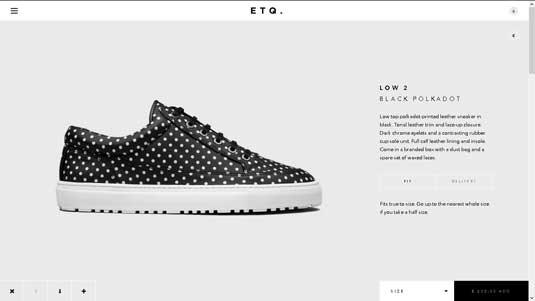
\includegraphics[width=8.0cm,height=4.0cm]{img/minimalismo.jpg}\centering
\begin{itemize}
\item Estos postulados son válidos no sólo para la arquitectura sino para todos los objetos que rodean a los seres humanos: el diseño debía ponerse al servicio del uso y el estilo, depurarse hasta llegar al minimalismo.
\end{itemize}
\end{frame}

\subsection{Experiencia de Usuario (UX) vs Experiencia de Cliente (CX)}
%References frame
\begin{frame}
\frametitle{Experiencia de Usuario (UX) vs Experiencia de Cliente (CX)}
\begin{itemize}
\item La Experiencia de Usuario se refiere a la experiencia que tienen las personas al interaccionar con un determinado producto. Una buena experiencia de usuario conlleva a que se cumplan y se cubran las necesidades del usuario, cumpliéndose los objetivos para los que fue creada la web.
\item La Experiencia del Cliente engloba todas las interacciones que tiene una persona con una marca a través de los diferentes canales: la primera vez que compra en una web, la solución de algún problema por vía telefónica, la recepción de un paquete.
\end{itemize}
\end{frame}

\subsection{Una mala Experiencia de Usuario y una buena Experiencia de Cliente}
%References frame
\begin{frame}
\frametitle{Una mala Experiencia de Usuario y una buena Experiencia de Cliente}
\begin{itemize}
\item Imaginemos que has comprado una app deportiva que te ayudará a ponerte en forma. La primera vez que la usas te das cuenta de su uso es confuso y que no puedes acceder a las características que posee.
\item Por suerte, la aplicación tiene un teléfono de ayuda al usuario. Llamas y rápidamente te atiende un amable agente, que responde tus preguntas y te explica claramente cómo acceder a las características que necesitas. Todo está claro ahora y además, como compensación por las molestias, te hacen un pequeño regalo.
\item Este es un claro ejemplo de una mala Experiencia de Usuario y una buena Experiencia de Cliente. Sin embargo, aunque este caso se puede dar, es más común que se dé el caso contrario.
\end{itemize}
\end{frame}

\subsection{Una buena Experiencia de Usuario y una mala Experiencia de Cliente}
%References frame
\begin{frame}
\frametitle{Una buena Experiencia de Usuario y una mala Experiencia de Cliente}
\begin{itemize}
\item Supongamos que quieres reservar un hotel por Internet. Fácilmente accedes al sitio web y reservas las noches en las que estás interesado: encuentras los precios fácilmente, la navegación es clara, la carga de la página es rápida y el formulario de reserva es breve, la UX es buena y satisfactoria.
\item Sin embargo cuando llegas al hotel tu percepción cambia radicalmente: el trato del recepcionista deja mucho que desear y la habitación no está totalmente limpia como debería.
\item Mientras que un aspecto del hotel te ha resultado satisfactorio (la reserva online)  el resto de interacciones han sido nefastas, por lo que la Experiencia del Cliente no será muy positiva.
\end{itemize}
\end{frame}

\section{Accesibilidad}
%References frame
\begin{frame}
\frametitle{Accesibilidad}
\begin{itemize}
\begin{multicols}{2}
\item \textbf{Navegación Oculta}
\item \textbf{Popups}
\item \textbf{Heros Rotativos}
\item \textbf{Contraste}
\columnbreak
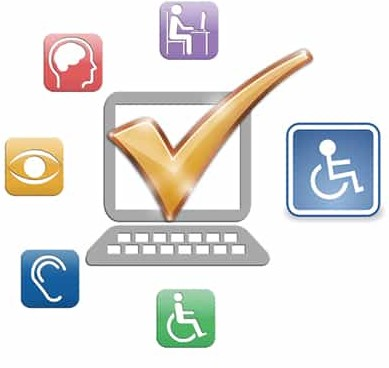
\includegraphics[width=5.0cm,height=5.0cm]{img/accesibilidad.jpg}
\end{multicols}
\end{itemize}
\end{frame}

\subsection{Navegacion Oculta}
%References frame
\begin{frame}
\frametitle{Áccesibilidad - Navegacion Oculta}
\begin{itemize}
\begin{multicols}{2}
\item \textbf{Menús de navegación que aparecen ocultos a primera vista y que con un clic se deslizan o se abren. }
\item \textbf{La navegación oculta ha prosperado y se ha convertido en una tendencia que ha venido para quedarse y ha evolucionado como recurso de diseño.}
\columnbreak
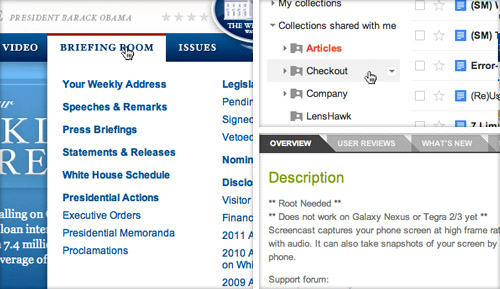
\includegraphics[width=5.0cm,height=5.0cm]{img/oculto.jpg}
\end{multicols}
\end{itemize}
\end{frame}

\subsection{Popups}
%References frame
\begin{frame}
\frametitle{Accesibilidad - Popups}
\begin{itemize}
\begin{multicols}{2}
\item \textbf{ Es una ventana nueva que aparece de repente en la pantalla de tu ordenador. }
\item \textbf{Los anuncios en pop-ups se utilizan mucho para hacer publicidad en la web.}
\columnbreak
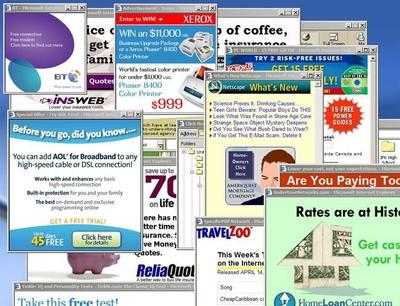
\includegraphics[width=5.0cm,height=5.0cm]{img/pop.jpg}
\end{multicols}
\end{itemize}
\end{frame}

\subsection{Popups(PAUTAS)}
\begin{frame}
\frametitle{Accesibilidad - Popups(PAUTAS)}
\begin{itemize}
\begin{multicols}{2}
\item \textbf{Solicitar una dirección de correo electrónico antes de la interacción}
\item \textbf{Mostrar una ventana emergente justo después de que el usuario inicia sesión}
\item \textbf{Mostrar una ventana emergente antes de que se cargue el contenido}
\columnbreak
\item \textbf{Pedir comentarios antes de que las personas hayan hecho algo significativo}
\item \textbf{Interrumpir a los usuarios para pedir comentarios durante las tareas críticas}
\item \textbf{Mostrar varias ventanas emergentes una tras otra}
\end{multicols}
\end{itemize}
\end{frame}

\subsection{Heros Rotativos}
%References frame
\begin{frame}
\frametitle{Accesibilidad - Heros Rotativos}
\begin{itemize}
\begin{multicols}{2}
\item \textbf{No esconder enlaces a secciones o a características importantes}
\item \textbf{El banner más importante en la primera posición}
\item \textbf{No deben rotar muy despacio}
\columnbreak
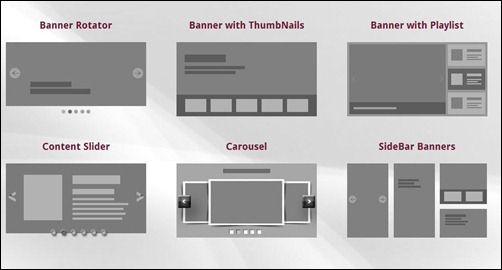
\includegraphics[width=5.0cm,height=5.0cm]{img/ban.jpg}
\end{multicols}
\end{itemize}
\end{frame}

\subsection{Contraste}
%References frame
\begin{frame}
\frametitle{Accesibilidad - Contraste}
\begin{itemize}
\begin{multicols}{2}
\item \textbf{No agregues colores solo para aparentar en tu diseño web}
\item \textbf{Gran claridad siempre que los resultados de búsqueda sean legibles}
\item \textbf{La paleta de colores del diseño material asegura la jerarquía visual}
\columnbreak
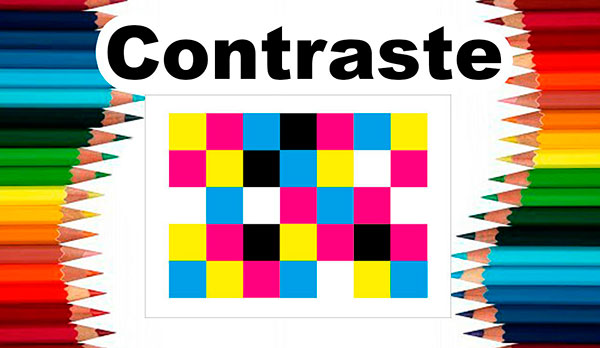
\includegraphics[width=5.0cm,height=5.0cm]{img/contraste.jpg}
\end{multicols}
\end{itemize}
\end{frame}


\section{Navegación}
\subsection{Un buen sistema de navegación}
%References frame
\begin{frame}
\frametitle{Navegación - Un buen sistema de navegación}
\begin{itemize}
\begin{multicols}{2}
\item \textbf{Página de inicio}
\item \textbf{Pie de página}
\item \textbf{Evitar páginas muertas}
\item \textbf{Enlazar siempre al índice}
\item \textbf{Ruta de acceso}
\item \textbf{Incluir un buscador}
\item \textbf{Una sección, un menú}
\item \textbf{Regla de los tres clicks}
\columnbreak
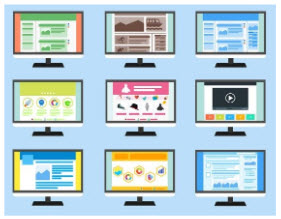
\includegraphics[width=5.0cm,height=5.0cm]{img/navegacion.jpg}
\end{multicols}
\end{itemize}
\end{frame}

\subsection{Sobrecarga de menú}
%References frame
\begin{frame}
\frametitle{Navegación - Sobrecarga de menú}
\begin{itemize}
\begin{multicols}{2}
\item \textbf{No sobrecargar de menús ni botones}
\item \textbf{Tener en cuenta los colores}
\item \textbf{Simplicidad}
\item \textbf{Visualmente atractivo}
\item \textbf{Buena descripción de los ítem del menú}
\columnbreak
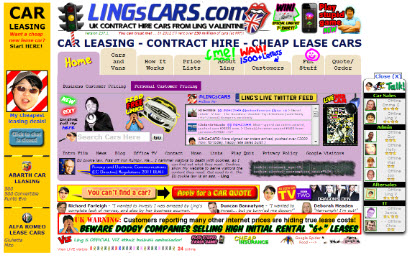
\includegraphics[width=5.2cm,height=4.5cm]{img/ejemplo.jpg}
\end{multicols}
\end{itemize}
\end{frame}

\subsection{Amplitud vs Profundidad}
%References frame
\begin{frame}
\frametitle{Navegación - Amplitud vs Profundidad}
\begin{itemize}
\begin{multicols}{2}
\item \textbf{Amplitud: cuanta información te muestra de un solo momento para llegar a la información.}
\item \textbf{Profundidad: cuantos clicks haces para llegar a la información.}
\columnbreak
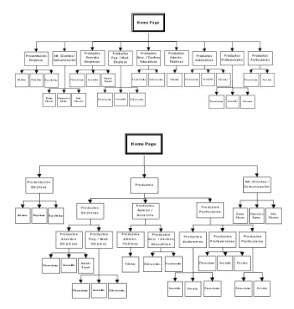
\includegraphics[width=5.2cm,height=5.0cm]{img/amplitud.jpg}
\end{multicols}
\end{itemize}
\end{frame}

\subsection{MegaMenu}
%References frame
\begin{frame}
\frametitle{Navegación - MegaMenu}
\begin{itemize}
\item Las opciones del mega menú se descubren pasando por encima, haciendo clic o con un toque (interfaz táctil)
\begin{multicols}{2}
\item \textbf{Un gran panel de navegación dividido en opciones de navegación}
\item \textbf{Opciones de navegación estructurada mediante maquetación, tipografía o iconos}
\item \textbf{Tiene que ser visible completamente de una vez, sin hacer scroll}
\item \textbf{Disposición horizontal (la más habitual) o vertical}
\columnbreak
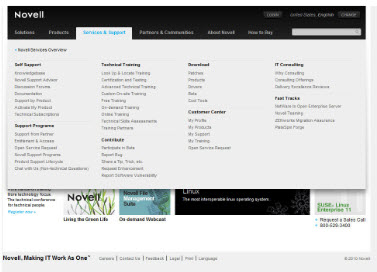
\includegraphics[width=5.2cm,height=5.5cm]{img/megamenu.jpg}
\end{multicols}
\end{itemize}
\end{frame}

\subsection{Breadcrumb}
%References frame
\begin{frame}
\frametitle{Navegación - Breadcrumb}
\begin{itemize}
\begin{multicols}{2}
\item \textbf{Si el sitio web tiene una estructura lineal con no más de dos niveles de páginas, no es necesario el uso de breadcrumbs}
\item \textbf{Mejor experiencia de usuario}
\item \textbf{Mejor estructura de enlaces internos}
\item \textbf{Fragmentos de búsqueda irresistibles}
\columnbreak
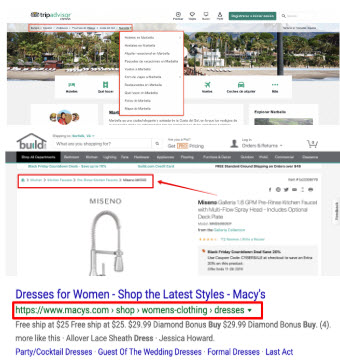
\includegraphics[width=5.2cm,height=5.5cm]{img/breadcrum.jpg}
\end{multicols}
\end{itemize}
\end{frame}

\subsection{Menu Hamburger}
%References frame
\begin{frame}
\frametitle{Navegación - Menu Hamburger}
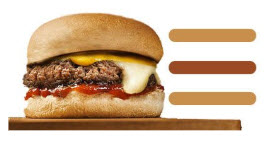
\includegraphics[width=1.7cm,height=1.7cm]{img/hamburguesa.jpg}\centering
\begin{itemize}
\begin{multicols}{2}
\item \textbf{Ventajas}
\item \textbf{El menú no entorpezca la experiencia de usuario cuando navega desde su smartphone o tablet.}
\item \textbf{Solo aparece cuando el usuario le hace un clic con el dedo.}
\columnbreak
\item \textbf{Desventajas}
\item \textbf{El usuario tiene que hacer un clic para mostrar los elementos del menú.}
\item \textbf{Reduce la experiencia deL usuario, ya que se convierte en un paso más para llegar a su destino.}
\item \textbf{Oculta la información a los usuarios y la navegación.}
\end{multicols}
\end{itemize}
\end{frame}

\subsection{Otros caminos para no usar menu Hamburger}
%References frame
\begin{frame}
\frametitle{Navegación - Otros caminos para no usar menu Hamburger}
\begin{multicols}{2}
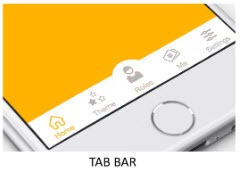
\includegraphics[width=5.5cm,height=5.5cm]{img/tabbar.jpg}
\columnbreak
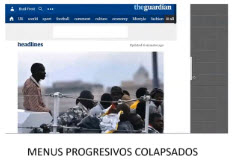
\includegraphics[width=5.5cm,height=5.5cm]{img/colapsados.jpg}
\end{multicols}
\end{frame}

\section{Contenidos}
\subsection{Espacios}
%References frame
\begin{frame}
\frametitle{Contenidos - Espacios}
\begin{itemize}
\begin{multicols}{2}
\item \textbf{Mito: Las personas no scrollean}
\item \textbf{La mayoría de páginas que tienen un contenido amplio suelen usar organizadores de información. Por ejemplo, Wikipedia, en su versión móvil utiliza un acordeón.}
\item \textbf{Estadísticamente se comprobó que a las personas no le importa mucho el hecho de que tengan que desplazarse hacia abajo de la página para buscar información}
\columnbreak
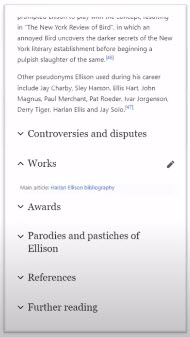
\includegraphics[width=5.0cm,height=6.5cm]{img/espacios.jpg}
\end{multicols}
\end{itemize}
\end{frame}

\subsection{Above the fold vs Beyond the fold}
%References frame
\begin{frame}
\frametitle{Contenidos - Above the fold vs Beyond the fold}
\begin{itemize}
\begin{multicols}{2}
\item \textbf{Basado en los titulares de los periódicos, el trabajo de ese espacio es importante al momento de querer hacer visible la información más relevante.}
\item \textbf{A pesar de esto, no significa un punto determinante al momento de atraer al lector.}
\item \textbf{La información brindada suele ubicarse "beyond the fold", por lo que los lectores buscan mayormente en esa zona.}
\columnbreak
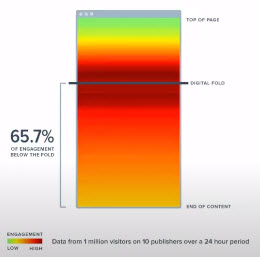
\includegraphics[width=5.0cm,height=6.5cm]{img/fold.jpg}
\end{multicols}
\end{itemize}
\end{frame}

\subsection{Espacios en blanco}
%References frame
\begin{frame}
\frametitle{Contenidos - Espacios en blanco}
\begin{itemize}
\begin{multicols}{2}
\item \textbf{El espacio en blanco es parte del diseño y de la experiencia de usuario}
\item \textbf{A veces menos es más}
\columnbreak
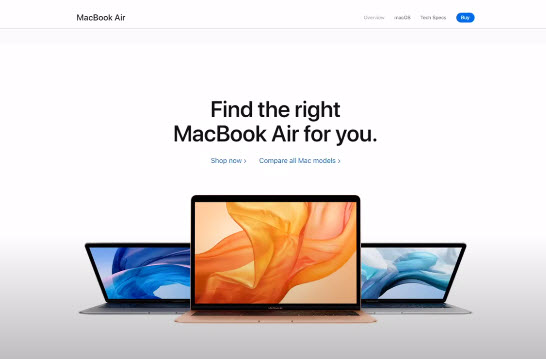
\includegraphics[width=5.0cm,height=3.0cm]{img/mac.jpg}
\end{multicols}
\end{itemize}
\end{frame}

\subsection{Espacio Macro}
%References frame
\begin{frame}
\frametitle{Contenidos - Espacio Macro}
\begin{itemize}
\begin{multicols}{2}
\item \textbf{Es el espacio entre distintos elementos que contiene la página}
\item \textbf{Si una imagen no cumple una función, es una decoración}
\columnbreak
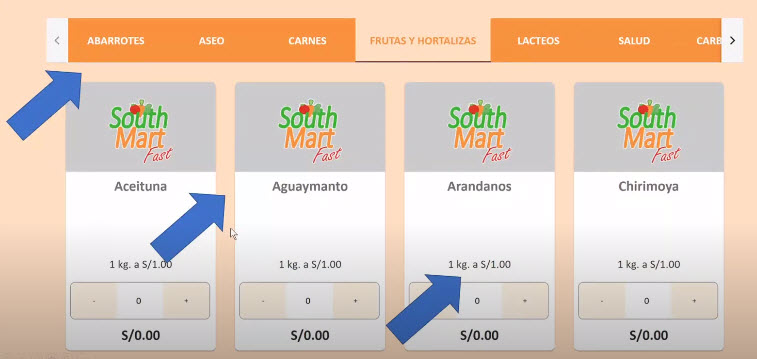
\includegraphics[width=5.0cm,height=3.0cm]{img/macro.jpg}
\end{multicols}
\end{itemize}
\end{frame}

\subsection{Espacio Micro}
%References frame
\begin{frame}
\frametitle{Contenidos - Espacio Micro}
\begin{itemize}
\begin{multicols}{2}
\item \textbf{Es el espacio que se encuentra entre los textos y las palabras}
\item \textbf{El 90\% de diseño es la tipografía, y el otro 90\% son los espacios en blanco (Jeffrey Zeldman)}
\columnbreak
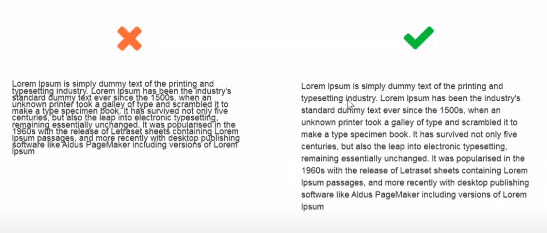
\includegraphics[width=5.0cm,height=3.0cm]{img/micro.jpg}
\end{multicols}
\end{itemize}
\end{frame}

\section{Textos}
%References frame
\begin{frame}
\frametitle{Textos}
\begin{itemize}
\begin{multicols}{2}
\item \textbf{Idea de las Jerarquías}
\item \textbf{Alineación}
\begin{itemize}
    \item \textbf{El problema de la justificación en textos grandes}
    \item \textbf{Comodidad de lectura}
\end{itemize}
\item \textbf{Ancho de lineal ideal}
\begin{itemize}
    \item \textbf{Entre 60 - 70 caracteres}
\end{itemize}
\item \textbf{MAYUSCULAS y minusculas}
\begin{itemize}
    \item \textbf{Priorización de contenidos}
    \item \textbf{Uniformidad}
\end{itemize}
\item \textbf{Otros Idiomas}
\columnbreak
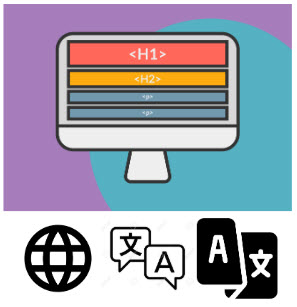
\includegraphics[width=5.0cm,height=6.0cm]{img/texidio.jpg}\centering
\end{multicols}
\end{itemize}
\end{frame}

\begin{frame}
\frametitle{Textos}
\begin{itemize}
\begin{multicols}{2}
\item \textbf{Legibilidad}
\begin{itemize}
    \item \textbf{Susceptibilidad a ser escaneado o ojeado}
    \item \textbf{Color con suficiente contraste, fuente simple y uso de técnicas de formato}
\end{itemize}
\item \textbf{Color}
\begin{itemize}
    \item \textbf{Número de colores limitados}
    \item \textbf{Codificacion de informacion sin contradicciones}
    \item \textbf{Combinación de colores compatibles}
    \item \textbf{Saturación con cautela}
\end{itemize}
\columnbreak
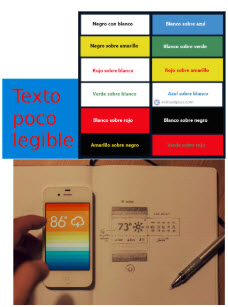
\includegraphics[width=5.0cm,height=6.0cm]{img/colores.jpg}\centering
\end{multicols}
\end{itemize}
\end{frame}

\section{Propuesta}
%References frame
\begin{frame}
\frametitle{Propuesta}
\begin{itemize}
\begin{multicols}{2}
\item \textbf{El grupo propone como trabajo futuro, analizar el estado de diseño de las páginas que ofrece la Universidad Nacional de San Agustín de Arequipa, brindando mejoras a los posibles errores que presente.}
\item \textbf{Complementando el punto anterior, desarrollar alguna metodología de evaluación conjunta a todos los aspectos mencionados.}
\columnbreak

\includegraphics[width=5.0cm,height=6.0cm]{img/aplicacion.jpg}
\end{multicols}
\end{itemize}
\end{frame}

\section{References}
%References frame
\begin{frame}
\frametitle{References}
\begin{itemize}
\item https://time.com/12933/what-you-think-you-know-about-the-web-is-wrong/
\item https://uxmyths.com/post/654047943/myth-people-dont-scroll
\item https://www.idento.es/blog/desarrollo-web/experiencia-usuario-vs-experiencia-cliente/
\item https://trello.com/b/fKFrCHMx/exposicion-hci
\item https://www.ttandem.com/blog/5-claves-para-conseguir-una-experiencia-de-usuario-positiva-en-tu-sitio-web/
\end{itemize}
\end{frame}
%References frame
\begin{frame}
\frametitle{References}
\begin{itemize}
\item https://www.mcarmendealba.com/wp-content/uploads/2018/05/Experiencia\_de\_Usuario\_Principios-y-metodos.pdf 
\item https://www.lawebera.es/diseno-web/menu-navegacion.php#que-debe-tener-un-buen-sistema-de-navegacion-web
\item https://www.torresburriel.com/weblog/2017/03/31/mega-menus-una-buena-navegacion/
\item https://www.youtube.com/watch?v=nNx2T-yU0NI&t=1812s
\end{itemize}
\end{frame}

\end{document}